%% LyX 2.0.6 created this file.  For more info, see http://www.lyx.org/.
%% Do not edit unless you really know what you are doing.
\documentclass[11pt]{article}
\usepackage[latin9]{inputenc}
\usepackage{listings}
\usepackage{float}
\usepackage{graphicx}

\makeatletter

%%%%%%%%%%%%%%%%%%%%%%%%%%%%%% LyX specific LaTeX commands.
%% Because html converters don't know tabularnewline
\providecommand{\tabularnewline}{\\}

%%%%%%%%%%%%%%%%%%%%%%%%%%%%%% User specified LaTeX commands.

\usepackage{fullpage}\usepackage{morefloats}\usepackage{url}\usepackage{pdftexcmds}\usepackage{listings}
\let\textquotedbl="

\makeatother

\begin{document}

\title{Processing USPTO Patent Data}


\author{Gabe Fierro\\
 Coleman Fung Institute for Engineering Leadership\\
 UC Berkeley\\
 \texttt{fierro@eecs.berkeley.edu}}


\date{\today}

\maketitle
 
\begin{abstract}
We describe a completely automated data process designed to consume
weekly releases of patent grants and applications distributed by the
United States Patent and Trademark Office (USPTO). The process downloads
and unpacks the zipped distribution files, parses the raw data into
a SQL database, and performs various disambiguations and statistical
calculations on the database. 
\end{abstract}

\section{Introduction}

There was a big database which had a lot of information related to patents. This database was divided into tables each of which contained different parts of information (patent information, inventor information, assignee information, lawyer information, etc.). However, before creating this interface, the only way to access this information was by making SQL queries. This required login credentials to the MySQL database, and SQL query forming expertise. To give a person without these privileges access to this information, we needed a web page where users could select what information they want from this database.

	The goal was to make a user friendly web interface which allowed users to select what rows they wanted from the tables in the database, specify any filters they wanted to specify for these rows, enter their email address, and specify the format in which they wanted the information (CSV, TSV, or SQLITE3). To do this, we selected to use the Django~\cite{django} framework because it was easy to install and learn. And then, to run the query itself, we used an external python file that imported the Django settings and just ran jobs if any were available (or sleep for some specific amount of seconds if no jobs were available). Our final goal was to make an app that would do this sort of forms to queries transformation on any database with minimal changes to the files included in the app.  


\section{Processing Workflow}

\begin{figure*}
\center
\includegraphics[width=.8\textwidth]{figs/dataprocess}
\caption{Full patent data process flow}
\label{fig:dataprocess}
\end{figure*}

The Fung Institute has developed a robust and fully automated toolchain for processing and providing high quality patent data intended for research, as illustrated in Figure~\ref{fig:dataprocess}.

As data is downloaded from the USPTO weekly patent releases, it is parsed, cleaned and inserted into a SQL database. From this database, assignee and lawyer disambiguations are performed and the patents are geocoded with a location-based disambiguation. The output data from these processes are combined with the historical data from the Harvard Dataverse Network into a single consolidated database. From this database, an inventor-level disambiguation can be performed, and various applications can take advantage of the completed data. 


\section{Data Sources}

The unified patent dataset is composed of processed data from two
separate sources: the Harvard Dataverse Network (DVN)~\cite{disambiguation}
collection of patent data from 1975 through 2010 and the weekly distributions
of Google-hosted USPTO records~\cite{googlefiles}\cite{googlefiles-applications}.


\subsection{Harvard DVN}

The Harvard DVN patent database consists of data drawn from the National
Bureau of Economic Research (NBER), weekly distributions of patent
data from the USPTO, and to a small extent, the 1998 Micropatent CD
product~\cite{micropatent}. The schema of the database can be found
in the Appendix.

While the Harvard DVN patent database was, prior to the UC Berkeley
patent database, the most extensively complete amalgamation of United
States patent data, it is not without its problems. Firstly, there
is little information as to the actual meanings of the columns in
the databases. Without sufficient prior knowledge of patent structure,
it is difficult to glean the semantic significance of each column.
The names alone are often abbreviated and hard to discern. Secondly,
because the DVN database is a combination of several sources into
a single database schema, certain patent entries from NBER and Micropatent
are incomplete where their data source did not provide all the requisite
data. The data obtained from the weekly distributions suffers from
being made available in several different formats. The parser that
was developed to handle the data is overly complicated and does not
handle edge cases well, resulting in missing patent metadata where
the parser did not account for a subtle change in format~\cite{oldparser}.
This is analyzed in greater detail below.


\subsection{USPTO Weekly Distributions}

\begin{table*}[t]
\center %
\begin{tabular}{|l|l|}
\hline 
Time Span  & Data Format \tabularnewline
\hline 
-1974  & paper-based \tabularnewline
1975  & unknown. Data obtained from Micropatent \tabularnewline
1976 - 2001  & Green Book (CITE) APS key-value \tabularnewline
2001  & SGML ST. 32 v2.4 \tabularnewline
2002 - 2004  & Red Book (CITE) XML ST. 32 v2.5 \tabularnewline
2005  & Red Book XML ST. 36 (ICE) v4.0 \tabularnewline
2006  & Red Book XML ST. 36 (ICE) v4.1 \tabularnewline
2007 - 2012  & Red Book XML ST. 36 (ICE) v4.2 \tabularnewline
2013  & Red Book XML ST. 36 (ICE) v4.3 \tabularnewline
2013 -  & Red Book XML v4.4 \tabularnewline
\hline 
\end{tabular}\caption{Table of USPTO grant data formats}


\label{fig:grantformats} 
\end{table*}
\begin{table*}[t]
\center %
\begin{tabular}{|l|l|}
\hline 
Time Span  & Data Format \tabularnewline
\hline 
-2001 & paper-based \tabularnewline
2001  & XML ST. 32 v1.5\tabularnewline
2002 - 2004  & Red Book (CITE) XML ST. 32 v1.6 \tabularnewline
2005 & Red Book XML ST. 36 (ICE) v4.0\tabularnewline
2006 & Red Book XML ST. 36 (ICE) v4.1 \tabularnewline
2007 - 2012 & Red Book XML ST. 36 (ICE) v4.2 \tabularnewline
2013 -  & Red Book XML v4.3\tabularnewline
\hline 
\end{tabular}\caption{Table of USPTO grant data formats}


\label{fig:applicationformats} 
\end{table*}


The USPTO distributions take the form of zip archives containing concatenated
XML (Extensible Markup Language) documents, each of which contains
the full text of each patent grant and patent application issued every
week. Prior to 1975, the USPTO used a purely paper-based system before
transitioning to a raw-text key-value and later SGML-based key-value
store %
\footnote{Standard Generalized Markup Language%
}. Patent documents were made available in the XML format starting
in 2001. Although this data is made freely available, the fact that
digital USPTO patent data spans eight different formats and occupies
more than 70 GB (compressed) over the 37 years of its existence makes
rendering the data into an amenable form a nontrivial problem (see
Table~\ref{fig:grantformats} and Table~\ref{fig:applicationformats}).
Patent application data, though only available in a digital format
back to 2001, is nonetheless available in six different formats~\cite{xmlresources}~\cite{xmlretrospective}.
 


\section{Parsing}

All of the conversion from HTML form to a SQL query is done in \verb`batchsql/models.py`. All of the form variables are given to the TestQuery class through the post variable that we get from django. In post, all the values entered by the user are stored as a dictionary in the form {“field-name”:”value”}. All form elements are broadly categorized into three types: 

\begin{enumerate}
\item Field Variables: These are the columns that the user wants information from. For example, Name of a Patent, or Name of the Inventor of the Patent.
\item Filter Variables: These are the filters specified by the user. They are mostly textboxes or select lists. If a user enters ‘TX’ under the Inventor’s location filter, then all the rows (in the columns specified by field variables) that have the inventor’s location as ‘TX’ will be returned.
\item Miscellaneous: The csrf token, the email address, the file type that the user wants the information in are considered as miscellaneous fields as models.py does not use these fields to make queries.
\end{enumerate}

	In models.py, we have a dictionary which maps the form elements’ names to (table,column) which they represent. For example, the Patent Title represents the patent table and the title column, and hence one of the entries in this dictionary will be \verb`‘pri-title’:(‘patent’, ‘title’)`(where ‘pri-title’ is the name of the field for Patent Title). All fields have a prefix of ‘f’ to separate them from filters. Converting the form elements is a 4 step process:

\begin{enumerate}
\item Get columns that the users want in their results and store it in a set. This is generated from the Field Variables.
\item Get the names of tables to be searched and store it in a set. This is generated from both the Field Variables and Filter Variables.
\item Get the filter conditions and store it in a set. This is generated from both the Field Variables (for cross-referencing between tables) and Filter Variables.
\item Loop through the above sets and construct a query of the structure\\
\end{enumerate}

\begin{center}
SELECT \{table.columns\} FROM \{tables\} WHERE \{filters\};
\end{center}

	Once this query is generated, it is stored in a local databse that stores the queued and completed job information, and then the \verb`run_jobs.py` file gets this query from this database and runs the jobs that have not yet been completed. It uses sqlalchemy~\cite{sqlalchemy} to connect  to and execute queries at the remote MySQL~\cite{mysql} database. 


\section{Database}

One of the main purposes of the patent processor project is to provide a usable
database of relevant patent data. This database should facilitate the retrieval
of patent records, citations, inventors, lawyers, assignees, and other
patent-related data. The linked nature of these types of records suggests that
a relational database model would be most suited to the data, which motivated
the decision to model patent data in SQL. SQL, or Structured Query Language, is
a language designed for managing data held in a relational database.

Because the majority of the data processing pipeline is written in Python, it
is hard to integrate otherwise easy-to-use SQL code. There are multiple flavors
of SQL -- among them, SQLite and MySQL. SQLite simplifies local development
because the whole database is represented as a single efficiently-sized file
that can be copied, moved and manipulated much like a traditional file.
However, it is hampered by a lack of support for more complex SQL features, and
has poor support for concurrent users (e.g. multiple processes attempting to
access the same database). MySQL offers advanced SQL features (such as
\verb`LEFT OUTER JOIN`) and scales to multiple users and large amounts of data
much easier than SQLite, but requires more specialized knowledge to use and
access. MySQL is more suited for production environments, whereas SQLite is
better for development. We want to be able to easily switch between these two
flavors of SQL depending on our purpose without having to develop multiple
branches of database integration.

\subsection{SQLAlchemy}

\begin{figure*}
\begin{lstlisting}
query = `select * from Patent where \
   number = ``%s''' % patent_number
result = connection.execute(query)
patent_id = result[3]
query = 'select * from assignee \
  where patent_id = ``%s''' % patent_id
connection.execute(query)
\end{lstlisting}
\label{fig:sql-assignee}
\caption{Finding assignees for a patent using traditional Python-SQL}
\end{figure*}

\begin{figure*}
\begin{lstlisting}
patent = session.query(Patent).
   filter_by(number = patent_number)
patent.assignees
\end{lstlisting}
\label{fig:sa-assignee}
\caption{Finding assignees for a patent using SQLAlchemy}
\end{figure*}

SQLAlchemy~\cite{sqlalchemy} is a Object Relational Mapper (ORM) for Python
that seeks to abstract away the differences between SQLite, MySQL, and other
SQL-based relational databases. The SQLAlchemy ORM maps Python classes to an
underlying SQL database such that the database can be manipulated as though it
were a native Python object. This means that the object model and the database
schema can be decoupled, effectively removing the need for separate lines of
development for each possible database engine.

Database-related code written using SQLAlchemy is much cleaner and easier to
work with than the traditional, kludgy idioms. In the case of SQLite, the
normal Python module requires the user to excute strings of SQL code:
\begin{lstlisting}
query = `select * from Patent where \
   number = ``%s''' % patent_number
connection.execute(query)
\end{lstlisting}

Not only does this require the programmer to know SQL syntax, but this paradigm
leaves the database open to SQL injection, wherein unintended and possibly
malicious code is executed on the SQL database. For example, here, we are
operating on the assumption that the variable \verb`patent_number` contains a
valid patent number. It could actually contain the string \verb`''; delete from Patent;--`,
which would terminate the original \verb`select` statement, delete
all entries from the Patent table, and then exit as though nothing had
happened. To avoid such attacks, it is necessary to sanitize all SQL strings
to make sure they contain valid and safe queries.

SQLAlchemy obviates the need to implement such verbose security methods. The
SQLAlchemy equivalent to the above query is:

\begin{lstlisting}
session.query(Patent).
   filter_by(number = patent_number)
\end{lstlisting}

Immediately, we can see that this code is much simpler and cleaner. When
SQLAlchemy accepts string input, as with the \verb`patent_number` variable
here, it automatically escapes all significant characters like semicolons and
apostrophes, essentially nullifying the possiblity of SQL injection attacks.

SQLAlchemy further simplifies the handling of foreign keys and complex joins
between tables, and can even implement these features over database engines
(such as SQLite) that do not normally have them. Consider
Figure~\ref{fig:sql-assignee} versus Figure~\ref{fig:sa-assignee}.

\subsection{Limitations}

The nice features of SQLAlchemy come at a price. The higher level interface to
the SQL database requires a nontrivial amount of bookkeeping. Foreign keys
lookups and checks introduce a certain amount of overhead, so when a process
loops through a list of database items, multiple SQL queries can be executed
against the backend for each object if the process asks for linked objects.

SQLAlchemy offers tools to help reduce the number of individual queries sent
to the underlying database, but there is an inescapable overhead to using an
ORM over the raw SQL.

\subsection{New Schema}

\begin{figure*}
    \center
    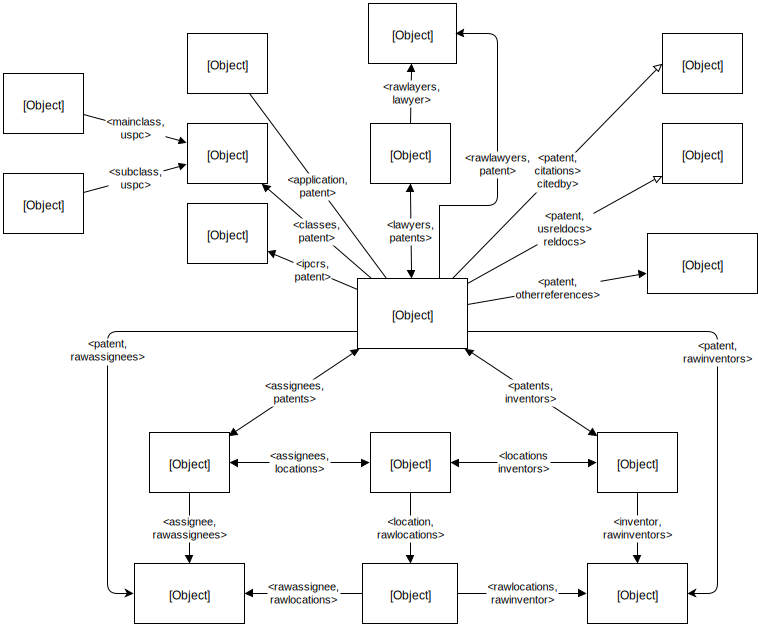
\includegraphics[width=.6\textwidth]{figs/database-simplified}
    \caption{High level view of new database schema}
    \label{fig:newschema}
\end{figure*}

We wanted to have a highly-linked database that would make it easy for
developers to access related information for a given set of patents. The DVN
schema, as described in the Appendix, does not take advantage of foreign key
relations, and places much manual burden on the user. This was a primary
motivating factor in our design, which is summarized in
Figure~\ref{fig:newschema}.

\subsection{Raw vs Processed}

If we examine the new database schema, for each of the \verb`inventor`,
\verb`lawyer`, \verb`location`, and \verb`assignee` tables, we can see a
``raw'' version (e.g. \verb`rawinventor`) and a plain version. The \verb`raw`
tables contain the inventor, lawyer, location and assignee records \emph{as
they appear in the USPTO files}, which means that the naming inconsistencies
and misspellings are preserved. These records are run through disambiguation
methods of various degrees of rigor, and the cleaned records are stored in the
plain tables. See below for a description of these disambiguation methods.

When the cleaned records are inserted, we link them to both the related patent
and the raw version using foreign keys in the database, so it is simple to
examine groups of related records. See Table~\ref{table:rawclean}.

\begin{table*}
\center
\begin{tabular}{| l | l | l |}
    \hline
    Table & Access & Value \\
    \hline
    Patent & \verb`patent` & US8434162 \\
    Inventor & \verb`patent.inventors[0]` & Thomas H. Stachler \\
    Raw Location & \verb`patent.inventors[0].rawlocation` & Deyton, OH, US \\
    Clean Location & \verb`patent.inventors[0].location` & Dayton, OH, US \\
    \hline
\end{tabular}
\caption{Accessing related raw and clean records. Note the spelling correction in the clean record}
\label{table:rawclean}
\end{table*}

 


\section{Disambiguations}

One of the primary problems with conducting meaningful research with
USPTO patent data is the high variability in quality. Cities are misspelled
or mislisted. Organizations are alternatively abbreviated and listed
in full with little modicum of consistency. Inventors, lawyers and
assignees will misspell their names, change their names and unpredictably
list their middle initials or names. The Berkeley patent database
provides facilities to account for these errors, and codifies the
disambiguation of such records in order to make possible their accurate
retrieval.


\subsection{Geocoding}

There are over 12 million locations listed in the USPTO patent weekly
downloads from 1975 to 2013, with 350,000 unique tuples of \verb`(city, state, country)`.
These tuples follow the typical motif of data problems in the rest
of the patent data: incorrect or nonstandard country codes, inconsistent
romanization of foreign locations and various misspellings. We resolved
the ambiguities in the location data using a propietary disambiguation
technique developed by Google. When new patent data is processed,
we run a series of data cleaning processes to correct for some of
the common errors, then cross reference with the lookup table~\cite{geotable}
obtained through the Google disambiguation.

A detailed analysis of the problems with USPTO location data and our
handling of locations can be found through a related Fung Institute
publication~\cite{geocoding}.

Locations are associated with assignees, inventors and lawyers. Typically,
a patent record's ``location'' is the location of the first inventor
listed on the patent.


\subsection{Assignees}

For a given patent, the assignees are the entities (either organizations
or individuals) that have property rights to the patent. The assignee
records are imperative for firm-level analysis of patent data, and
are used for tracking ownership of patents. The weekly releases of
patent documents only contain the original assignee of a patent when
it was initially granted.

However, it is difficult to obtain accurate results for simple (and
necessary) questions such as \emph{``which patents are owned by firm
X?''} because of the pandemic inconsistency of spellings. A cursory
search for assignee records that resemble General Electric yields
the following:
\begin{itemize}
\item General Electric Company 
\item General Electric 
\item General Electric Co.. 
\item General Electric Capital Corporation 
\item General Electric Captical Corporation 
\item General Electric Canada 
\item General Electrical Company 
\item General Electro Mechanical Corp 
\item General Electronic Company 
\item General Eletric Company 
\end{itemize}
This is not even a complete list of all the (mis)representations of
General Electric, but already we can see the potential issues with
trying to get accurate results.

We do not yet provide fully featured entity resolution for assignee
records, but we do maintain a preliminary disambiguation of the records
that corrects for minor misspellings. We do this by applying the Jaro-Winkler~\cite{jw}
string similarity algorithm to certain pairs of raw assignee records.
Two records that are within a certain bound of similarity are considered
the same, and are linked together.

It is not tractable to perform pairwise computation on each of the
5,850,531 raw assignee records in the database (at time of writing),
so we group the assignees by their first letter, and then perform
the pairwise comparisions within each of these blocks. This allows
us to hold a smaller chunk of the assignees in memory at each step,
with approximate accuracy.

First, all assignees are associated with a ``clean identifier'', which consists
of the organization name (or concatenated first and last names) of the
assignee, lower cased, with all non-letter and non-whitespace characters
removed. This simplifies the comparison process. Following this normalization,
all assignees are placed into a block according to the first letter of their clean
identifier.

Disambiguation occurs within blocks, resulting in a set of ``pools'' indexed by
a central assignee and containing assignees that are within some Jaro-Winkler
threshold of that central assignee. As assignees are popped off the end of the
list of non-disambiguated assignees, they are compared against each of the
central assignees. If their clean identifier is within the Jaro-Winkler
threshold of some central assignee, then the candidate is placed in that pool;
else, it is placed into a new pool of which it is the only member. This
continues until all assignees are placed into a pool. A record is chosen from
the pool to act as the dismbiguated record for that pool, and all rawassignees
are linked to that disambiguated record.

There is obvious room for improvement in this algorithm -- including more
global string comparisons and the leveraging of additioanl metadata to
further group and lump assignees -- but due to current computational
constraints, it is not possible to implement these changes within the current
framework. This disambiguation delivers a decent fix for the various misspellings
occurred in the database.

\subsection{Lawyers}

The raw lawyer records follow much of the same deficiencies in quality
as the assignee records. Again, we only offer a preliminary disambiguation
of lawyer records using the same algorithm as described above, but
future development will yield more accurate results.

The assignee disambiguation has yet to be implemented for the lawyer
record tables.

\subsection{Inventors}

We provide a polished disambiguation mechanism for inventor records.
Using the published name of an inventor, the patent technology class,
co-inventor names, published location and original assignee, we are
able to infer with more than 95\% accuracy which inventor records
are the same across all records in the patent database.

A detailed summary of our technique can be found through a related
Fung Institute publication~\cite{newdisambiguation}. 
 


\section{Statistics}

Many research applications of patent data require records from multiple
tables to be linked together: for instance, finding all citations
made to a patent, or finding all patents for an inventor. Due to the
size of the database, however, gathering all the requisite data and
linking it together takes a nontrivial amount of time. To facilitate
some common research vectors, we provide three tables of precompiled
statistics.

The \verb`FutureCitationRank` table contains the rank of each patent
by the number of future citations in each year. This answers the question
``in year X, patent number Y got Z citations. It was the Nth most
cited patent that year''.

The \verb`InventorRank` table contains the rank of each inventor
by how many patents they have been granted in a given year.

The \verb`CitedBy` table contains the direct mapping of a focal patent
to all patents that cite that patent. 


\section{Relationships}

Here we include entity-relationship diagrams (ERDs) that focus on subsets of the database, to better explain the one-to-many and one-to-one connections between tables in the database. A table is indicated by a box (the name of the table is in the header), and connections between tables are indicated by dotted lines. A dotted line with a dot at either end indicates a \textbf{one-to-one} relationship, meaning that the rows in one table map perfectly onto the rows in the other table without overlap. A dotted line with a fork at one end indicates a \textbf{one-to-many} relationship, where the rows of the ``one'' table potentially map onto several rows of the ``many'' table.

\subsection*{Patent Attributes}

As seen below, each patent has a one-to-many relationship with its citations, classes, claims and application records. Citations (\verb`uspatentcitation`, \verb`foreigncitation`, \verb`usapplicationcitation` and \verb`otherreference`) are listed in the database in the same order they are listed in the patent file (as indicated by the \verb`sequence` column in those tables). This is also the case for claims in the \verb`claim` table. Patent classifications exist in the \verb`uspc` table, and are listed in order by the \verb`sequence` column, separated into main- and sub-classifications. Each patent also has an entry in the \verb`application` table, which contains metadata about the related application for the granted patent document, including filing date and application number. This application number can be used as a foreign key into the application database to obtain information for the inventors, claims, etc listed on the application document.

\begin{figure*}[!htbp]
\includegraphics[width=\linewidth]{figs/Patentattributes}
\caption{Patents with citations, claims, applications and classes}
\end{figure*}

\subsection*{Patent Entities}

Here we explore the relationships between patents and inventors, lawyers and assignees.  Patents have \emph{many} \verb`rawlawyer`s, \verb`rawinventor`s and \verb`rawassignee`s. These relations are pulled directly from the USPTO XML files, that is, an instance of a \verb`rawinventor` belongs to a particular instance of a \verb`patent`, and no other records. As we will explore below, each of the \verb`rawlawyer`, \verb`rawinventor` and \verb`rawassignee` records is linked to a disambiguated record of the same type (\verb`rawassignee` to \verb`assignee`, for example).

\begin{figure*}[!htbp]
\includegraphics[width=\linewidth]{figs/Patententities}
\caption{Patents with Inventors, Assignees and Lawyers}
\end{figure*}

\subsection*{Inventors}

Expanding upon the patent-entity diagram above, we look at how inventor-related records are treated in the database. Patents have multiple inventors (order is, again, indicated by the \verb`sequence` column in the \verb`rawinventor` table) that are placed in the \verb`rawinventor` table. When the inventor disambiguation is run, each \verb`rawinventor` is linked with a disambiguated \verb`inventor` record in the \verb`inventor` table. As indicated in the ERD below, multiple \verb`rawinventor`s can be associated with a single \verb`inventor`. Each \verb`rawinventor` record also has a \verb`rawlocation` record, which is the location of that inventor as listed on the associated patent. Likewise, each \verb`rawlocation` is linked with a disambiguated \verb`location` record in the \verb`location` table after the geolocation disambiguation is performed. The linking table \verb`location_inventor` maintains the \verb`rawinventor-rawlocation` pairing, but uses the disambiguated records instead. Currently, the table contains all unique pairs of \verb`inventor` and \verb`location` as listed together on a patent document, in the order from oldest patent to newest patent. Keep in mind that because not all raw locations have disambiguated locations, not all inventors will have disambiguated locations.The \verb`patent_inventor` linking table mirrors the relationship of \verb`rawinventor` to \verb`patent`, but uses the disambiguated inventor record.

\begin{figure*}[!htbp]
\includegraphics[width=\linewidth]{figs/Inventor}
\caption{Inventor-related tables}
\end{figure*}

\subsection*{Assignees}

The relationships between raw and disambiguated assignee records follow the same logic as the inventor records above.

\begin{figure*}[!htbp]
\includegraphics[width=\linewidth]{figs/Assignee}
\caption{Assignee-related tables}
\end{figure*}

\subsection*{Lawyers}

The relationships between raw and disambiguated lawyer records follow the same logic as the assignee and inventor records above, with the exception
that patent documents do not contain location information about lawyers.

\begin{figure*}[!htbp]
\includegraphics[width=.3\linewidth]{figs/Lawyer}
\caption{Lawyer-related tables}
\end{figure*}

\newpage

{ {\scriptsize{ \bibliographystyle{acm}
\bibliography{patentprocessor}
 }}}
\end{document}
